% Options for packages loaded elsewhere
\PassOptionsToPackage{unicode}{hyperref}
\PassOptionsToPackage{hyphens}{url}
%
\documentclass[
  12pt,
]{article}
\usepackage{lmodern}
\usepackage{amsmath}
\usepackage{ifxetex,ifluatex}
\ifnum 0\ifxetex 1\fi\ifluatex 1\fi=0 % if pdftex
  \usepackage[T1]{fontenc}
  \usepackage[utf8]{inputenc}
  \usepackage{textcomp} % provide euro and other symbols
  \usepackage{amssymb}
\else % if luatex or xetex
  \usepackage{unicode-math}
  \defaultfontfeatures{Scale=MatchLowercase}
  \defaultfontfeatures[\rmfamily]{Ligatures=TeX,Scale=1}
  \setmainfont[]{Times New Roman}
\fi
% Use upquote if available, for straight quotes in verbatim environments
\IfFileExists{upquote.sty}{\usepackage{upquote}}{}
\IfFileExists{microtype.sty}{% use microtype if available
  \usepackage[]{microtype}
  \UseMicrotypeSet[protrusion]{basicmath} % disable protrusion for tt fonts
}{}
\makeatletter
\@ifundefined{KOMAClassName}{% if non-KOMA class
  \IfFileExists{parskip.sty}{%
    \usepackage{parskip}
  }{% else
    \setlength{\parindent}{0pt}
    \setlength{\parskip}{6pt plus 2pt minus 1pt}}
}{% if KOMA class
  \KOMAoptions{parskip=half}}
\makeatother
\usepackage{xcolor}
\IfFileExists{xurl.sty}{\usepackage{xurl}}{} % add URL line breaks if available
\IfFileExists{bookmark.sty}{\usepackage{bookmark}}{\usepackage{hyperref}}
\hypersetup{
  pdftitle={Final Project: Patterns of Lemur Density in Ranomafana National Park, Madagascar},
  pdfauthor={Camille DeSisto, Andrea Gonzalez, Courtney Horn},
  hidelinks,
  pdfcreator={LaTeX via pandoc}}
\urlstyle{same} % disable monospaced font for URLs
\usepackage[margin=2.54cm]{geometry}
\usepackage{longtable,booktabs}
\usepackage{calc} % for calculating minipage widths
% Correct order of tables after \paragraph or \subparagraph
\usepackage{etoolbox}
\makeatletter
\patchcmd\longtable{\par}{\if@noskipsec\mbox{}\fi\par}{}{}
\makeatother
% Allow footnotes in longtable head/foot
\IfFileExists{footnotehyper.sty}{\usepackage{footnotehyper}}{\usepackage{footnote}}
\makesavenoteenv{longtable}
\usepackage{graphicx}
\makeatletter
\def\maxwidth{\ifdim\Gin@nat@width>\linewidth\linewidth\else\Gin@nat@width\fi}
\def\maxheight{\ifdim\Gin@nat@height>\textheight\textheight\else\Gin@nat@height\fi}
\makeatother
% Scale images if necessary, so that they will not overflow the page
% margins by default, and it is still possible to overwrite the defaults
% using explicit options in \includegraphics[width, height, ...]{}
\setkeys{Gin}{width=\maxwidth,height=\maxheight,keepaspectratio}
% Set default figure placement to htbp
\makeatletter
\def\fps@figure{htbp}
\makeatother
\setlength{\emergencystretch}{3em} % prevent overfull lines
\providecommand{\tightlist}{%
  \setlength{\itemsep}{0pt}\setlength{\parskip}{0pt}}
\setcounter{secnumdepth}{5}
\ifluatex
  \usepackage{selnolig}  % disable illegal ligatures
\fi

\title{Final Project: Patterns of Lemur Density in Ranomafana National
Park, Madagascar}
\usepackage{etoolbox}
\makeatletter
\providecommand{\subtitle}[1]{% add subtitle to \maketitle
  \apptocmd{\@title}{\par {\large #1 \par}}{}{}
}
\makeatother
\subtitle{\url{https://github.com/ag522/LemurProject_DeSisto_Gonzalez_Horn.git}}
\author{Camille DeSisto, Andrea Gonzalez, Courtney Horn}
\date{}

\begin{document}
\maketitle

\newpage
\tableofcontents 
\newpage
\listoftables 
\newpage
\listoffigures 
\newpage

\hypertarget{rationale-and-research-questions}{%
\section{Rationale and Research
Questions}\label{rationale-and-research-questions}}

Madagascar is one of Earth's biodiversity hotspots that harbors high
levels of animal and plant endemism. Climate, land cover, and geography
determine patterns of plant community structure throughout the island
which, in turn, affects mammal diversity (Brown et al.~2015; Park \&
Razafindratsima 2019). Lemurs, Madagascar's most prominent group of
frugivores by both biomass and species richness, play a critical role in
seed dispersal and related processes and are important cultural icons
(Wright et al.~2005). However, 91\% of lemurs are threatened with
extinction due to anthropogenic disturbances (Schwitzer et al.~2014;
Razafindratsima et al.~2013).

Lemur habitat use is dependent on plant resource availability (Overdorff
1996), which is mediated by landscape-level characteristics such as
roughness and slope. In fact, food trees are stronger predictors of
lemur occurrence than climate (Herrera et al.~2017). Lemurs use
trait-based cues to select fruits (Valenta et al.~2013; Overdorff 1996).
For example, size matching, whereby large fruits are typically dispersed
by large vertebrates, is an essential phenomenon in driving
plant-frugivore interactions (Lim et al.~2020). Plant nutrient content
may also be an important factor in influencing frugivory interactions in
tropical forests. For example, Madagascar is the only region where there
is a significant relationship between fruit protein and the degree of
frugivory among primate communities (Donati et al.~2017). Additionally,
the average percentage of fruit nitrogen content in Madagascar is lower
than the minimum nitrogen requirement for primates, suggesting that the
low protein availability in Malagasy fruits is particularly important in
shaping lemur communities (Donati et al.~2017).

In this project, we examine a suite of environmental factors in relation
to lemur densities in Ranomafana National Park, Madagascar. We seek to
identify patterns in lemur densities throughout the park and examine
potential causes of these patterns.We predict that lemur densities are
negatively related to landscape roughness and slope and reward
regulation causes positive relationships between animal densities and
fruit nutrient contents. This research addresses three main hypotheses:
1) because different lemur species have specific responses to
environmental cues based on their life history traits, we hypothesize
that lemur densities among different sites and species are significantly
different; 2) we expect that both landscape-level characteristics and
plant functional traits act together to drive lemur densities throughout
a national park in Madagascar; and, 3) we hypothesize that different
species have distinct relationships between their individual densities
and habitat variables.

\newpage

\hypertarget{dataset-information}{%
\section{Dataset Information}\label{dataset-information}}

Data for this project were collected by James Herrera and Camille
DeSisto, as a part of a larger project aimed at investigating
plant-animal interactions in Madagascar's eastern rainforests. Field
data were collected by James Herrera and his colleagues in the montane
evergreen rainforest of Ranomafana National Park in southwestern
Madagascar. They conducted diurnal and nocturnal lemur surveys at five
sites (Ampatsoana, Maharira, Miaranony, Valohoaka, and Vohiparara)
between 2011 and 2014. Diurnal lemur surveys were conducted at 31
transects among these five sites, whereas nocturnal lemur surveys were
conducted at 26 of these sites due to logistical constraints. Habitat
variables (slope, roughness, location, topogaphic position index,
elevation, flow direction, and aspect) were collected along each
transects. Additionally, vegetation data were collected from botanical
surveys every 100 m along each transect. Camille DeSisto calculated
lemur densities using a distance sampling and model averaging approach
that jointly modeled for detection and density, using the R packages
``unmarked'' and ``MuMln'' (Fiske \& Chandler 201; Barton 2020; Figure
1). Trait data were previously collected from the literature and mean
trait values were calculated for each transect as part of the larger
research project.

Upon the start of this final project for ENV872, the dataset was already
clean and did not require much additional wrangling to be used for our
spatial visualization or linear models. However, we did use data
wangling to summarize the transects by group in order to conduct the
analysis of variance. In total, there are 11 plant functional trait
variables and 5 habitat variables per transect, in addition to the
predicted densities per lemur species (Table 1). Additional information
on the variables is available in the metedata file in the Github
repository. We also created a Transect Map App to better visualize the
data by species and site, as well as allowing the user to select a
variable and visualize it's relationship with population density for a
particular species per site. This application is available in out github
repository.

\newpage

\hypertarget{exploratory-analysis}{%
\section{Exploratory Analysis}\label{exploratory-analysis}}

We conducted an exploratory analysis of our data visually using a
heatmap to show differences in lemur densities among the different
transects and species (Figure 1). Visualizations in throughout this
project were conducted using the ``ggplot2'' package (Wockham 2016).
Additionally, we calculated summary statistics for the numeric habitat
variables in our dataset, as well as lemur densities (Table 1). Details
on the variables are available in the metedata file on the Github
repository.

\begin{figure}

{\centering 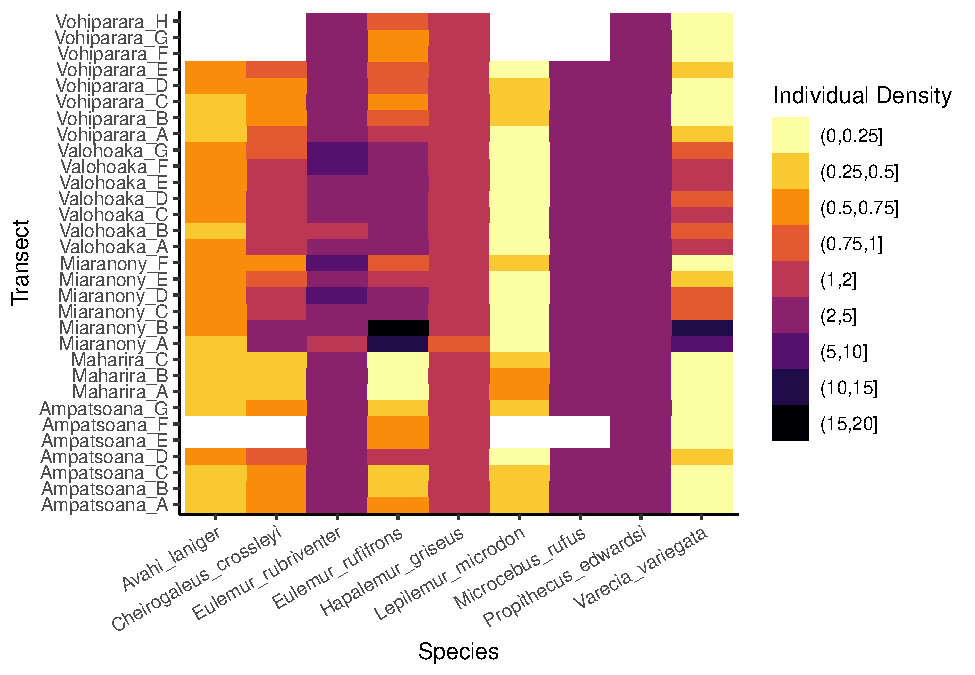
\includegraphics{project_draft_2_files/figure-latex/unnamed-chunk-2-1} 

}

\caption{Heat map of lemur densities at each project transect site}\label{fig:unnamed-chunk-2}
\end{figure}
\newpage

\begin{longtable}[]{@{}lrrrr@{}}
\caption{Summary Statistics for Transect-Level Variables}\tabularnewline
\toprule
& Maximum & Minimum & Mean & Standard Deviation\tabularnewline
\midrule
\endfirsthead
\toprule
& Maximum & Minimum & Mean & Standard Deviation\tabularnewline
\midrule
\endhead
LogFruitLength & 3.0367699 & 2.5481124 & 2.7884419 &
0.1078722\tabularnewline
LogFruitWidth & 2.8735245 & 2.4061911 & 2.6418949 &
0.1105788\tabularnewline
LogSeedLength & 2.4618778 & 1.8435241 & 2.2224035 &
0.1463275\tabularnewline
LogSeedWidth & 2.1370075 & 1.5738239 & 1.9532329 &
0.1329052\tabularnewline
LogSugar & 2.6292634 & 2.0849150 & 2.3969571 & 0.1121973\tabularnewline
LogFat & 1.8455284 & 1.5255786 & 1.6830810 & 0.0767810\tabularnewline
LogProtein & 4.2689341 & 3.2368227 & 3.7342967 &
0.2510554\tabularnewline
LogNitrogen & 0.9160242 & 0.7243437 & 0.8042614 &
0.0578926\tabularnewline
LogTannins & 0.1913672 & 0.0687408 & 0.1419214 &
0.0294709\tabularnewline
SLA & 2.4679473 & 2.2134377 & 2.3677036 & 0.0578060\tabularnewline
WD & 0.5986437 & 0.5414205 & 0.5804747 & 0.0101335\tabularnewline
Tpi & 73.7500000 & -206.7500000 & -0.3527992 & 60.5243149\tabularnewline
Roughness & 529.0000000 & 34.0000000 & 205.0308880 &
151.3989769\tabularnewline
Slope & 13.5005877 & 0.3904947 & 4.2638428 & 3.6935512\tabularnewline
Aspect & 280.1872004 & 9.7805570 & 135.9507256 &
67.2499763\tabularnewline
Flowdir & 64.0000000 & 1.0000000 & 6.2355212 & 10.1291339\tabularnewline
Density & 17.9717477 & 0.0566592 & 1.7848451 & 2.0068795\tabularnewline
\bottomrule
\end{longtable}

\newpage

\hypertarget{analysis}{%
\section{Analysis}\label{analysis}}

\hypertarget{question-1-are-there-significant-differences-in-lemur-densities-among-the-different-sites-and-among-the-different-species-if-so-how-can-the-sites-and-species-be-grouped-to-reflect-the-patterns-in-densities}{%
\subsection{Question 1: Are there significant differences in lemur
densities among the different sites and among the different species? If
so, how can the sites and species be grouped to reflect the patterns in
densities?}\label{question-1-are-there-significant-differences-in-lemur-densities-among-the-different-sites-and-among-the-different-species-if-so-how-can-the-sites-and-species-be-grouped-to-reflect-the-patterns-in-densities}}

First, we conducted a one-way analysis of variance (ANOVA) on lemur
population density by site using the ``aov'' function in the R general
interface. Next, we completed a post-hoc Tukey HSD test to determine
pairwise differences between the sites using the ``TukeyHSD'' function
from the R general interface. Then, we conducted a HSD post-hoc test
from the R package ``agricolae'' (de Mendiburu 2020) to categorize the
sites into groups based on their lemur densities. After these analyses
of the sites, we repeated the process between lemur species rather than
sites to determine if there are significant differences in densities
depending on the particular species.

\hypertarget{question-2-what-variables-are-related-to-differences-in-lemur-densities}{%
\subsection{Question 2: What variables are related to differences in
lemur
densities?}\label{question-2-what-variables-are-related-to-differences-in-lemur-densities}}

Next, we analyzed what transect-level habitat variables are
significantly related to lemur densities. After an exploratory
correlation plot to determine the correlations between the habitat
variables, we conducted linear mixed effects models using the ``lmer''
function in the R package ``lme4'' (Bates et al.~2015). We used lemur
density as the dependent variable and site-level habitat characteristics
(log fruit length, log fruit width, log seed length, log seed width, log
fruit nitrogen content, log tree tannin content, log fruit sugar
content, log fruit sugar content, log fruit protein content, latitude,
longitude, aspect, slope, and roughness) as the independent variables.
We conducted these models with both the transect and the lemur species
as random variables. In the first set of models we included site as an
independent variable, and in a second set of models we included it as a
random variable. We used a backwards stepwise approach to reduce the
models and conducted model selection via comparison of their Akaike
Information Criterion (AIC) values using the ``lrtest'' function in the
R package ``lmtest'' (Zeileis \& Horton 2002). Additionally, we
identified the R-squared values of the models using the
``r.squaredGLMM'' function in the R package ``MuMln'' (Barton 2020).

\hypertarget{question-3-what-transect-level-characteristics-and-plant-functional-traits-are-related-to-the-density-of-individual-lemur-species}{%
\subsection{Question 3: What transect-level characteristics and plant
functional traits are related to the density of individual lemur
species?}\label{question-3-what-transect-level-characteristics-and-plant-functional-traits-are-related-to-the-density-of-individual-lemur-species}}

The final step of our analyses was exploring the effects of habitat
variables for specific lemur species. To do this, we subset the data by
species and conducted linear models for four lemur species (\emph{Avahi
laniger, Eulemur rubriventer, Propithecus edwardsi}, and \emph{Lepilemur
microdon}) using the function ``lm'' from the R general interface. We
used density as the dependent variable and the aforementioned habitat
variables as independent variables. We chose to focus on these four
lemur species as case studies because we identified them as having
distinct densities based on the ANOVA and exploratory data analysis.
Further, we identified \emph{Avahi laniger} and \emph{Lepilemur
microdon} as having the two lowest mean densities of all species
included in our data, and we identified \emph{Propithecus edwardsi} and
\emph{Eulemur rubriventer} as having the two highest mean densities of
all species included in our data. Therefore, analyzing these four
species individually could provide us with insights into drivers of high
and low densities.

\hypertarget{results}{%
\section{Results}\label{results}}

\hypertarget{question-1-are-there-significant-differences-in-lemur-densities-among-the-different-sites-and-among-the-different-species-if-so-how-can-the-sites-and-species-be-grouped-to-reflect-the-patterns-in-densities-1}{%
\subsection{Question 1: Are there significant differences in lemur
densities among the different sites and among the different species? If
so, how can the sites and species be grouped to reflect the patterns in
densities?}\label{question-1-are-there-significant-differences-in-lemur-densities-among-the-different-sites-and-among-the-different-species-if-so-how-can-the-sites-and-species-be-grouped-to-reflect-the-patterns-in-densities-1}}

There is a significant difference in lemur densities between different
sites (F(4,254) = 3.469, p = 0.009; Figure 2). In particular, the
post-hoc Tukey HSD test revealed that there are significant differences
in densities between Miaranony and Ampatsoana (p = 0.0287), Miaranony
and Maharira (p = 0.031) and Vohiparara and Miaranony (p = 0.386) sites.
However, visual analysis of lemur densities via boxplots boxplots
(Figure 2) suggests that the higher lemur densities observed in
Miaranony and Valohoaka may be appributable to outliers. An HSD post-hoc
test from the R package ``agricolae'' (de Mendiburu 2020) indicates that
the sites can be categorized into two main groups according to their
lemur densities, with Miaranony in one group, Vohiparara, Ampatsona, and
Maharira in another group, and Valohoaka in both groups.

\begin{figure}
\centering
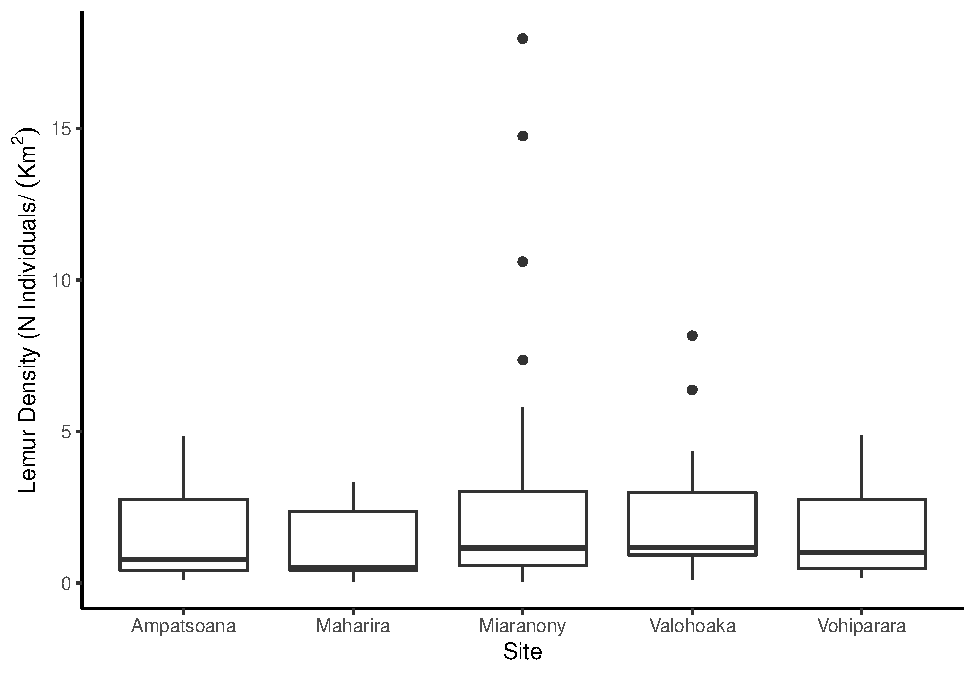
\includegraphics{project_draft_2_files/figure-latex/unnamed-chunk-9-1.pdf}
\caption{Boxplot of lemur densities at each sampling site.}
\end{figure}

There is also a significant difference in lemur densities between
different species (F (8,250) = 16.79, p = \textless2e-16; Figure 3). The
HSD post-hoc test indicates that lemur species can be categorized into
four main groups according to their density (Table 2).

\begin{longtable}[]{@{}ll@{}}
\caption{Groupings of lemur species according to their population
densities.}\tabularnewline
\toprule
\begin{minipage}[b]{(\columnwidth - 1\tabcolsep) * \real{0.79}}\raggedright
Group\strut
\end{minipage} &
\begin{minipage}[b]{(\columnwidth - 1\tabcolsep) * \real{0.21}}\raggedright
Average population Density\strut
\end{minipage}\tabularnewline
\midrule
\endfirsthead
\toprule
\begin{minipage}[b]{(\columnwidth - 1\tabcolsep) * \real{0.79}}\raggedright
Group\strut
\end{minipage} &
\begin{minipage}[b]{(\columnwidth - 1\tabcolsep) * \real{0.21}}\raggedright
Average population Density\strut
\end{minipage}\tabularnewline
\midrule
\endhead
\begin{minipage}[t]{(\columnwidth - 1\tabcolsep) * \real{0.79}}\raggedright
- \emph{Eulemur rubriventer},\emph{Propithecus
edwardsi},\emph{Microcebus rufus}\strut
\end{minipage} &
\begin{minipage}[t]{(\columnwidth - 1\tabcolsep) * \real{0.21}}\raggedright
2.72 - 3.80\strut
\end{minipage}\tabularnewline
\begin{minipage}[t]{(\columnwidth - 1\tabcolsep) * \real{0.79}}\raggedright
- \emph{Propithecus edwardsi},\emph{Microcebus rufus},\emph{Eulemur
rufifrons}\strut
\end{minipage} &
\begin{minipage}[t]{(\columnwidth - 1\tabcolsep) * \real{0.21}}\raggedright
2.31 - 3.03\strut
\end{minipage}\tabularnewline
\begin{minipage}[t]{(\columnwidth - 1\tabcolsep) * \real{0.79}}\raggedright
- \emph{Eulemur rufifrons} ,\emph{Hapalemur griseus}\strut
\end{minipage} &
\begin{minipage}[t]{(\columnwidth - 1\tabcolsep) * \real{0.21}}\raggedright
1.11 - 2.31\strut
\end{minipage}\tabularnewline
\begin{minipage}[t]{(\columnwidth - 1\tabcolsep) * \real{0.79}}\raggedright
- \emph{Hapalemur griseus},\emph{Varecia variegata },\emph{Cheirogaleus
crossleyi},\emph{Avahi laniger },\emph{Lepilemur microdon}\strut
\end{minipage} &
\begin{minipage}[t]{(\columnwidth - 1\tabcolsep) * \real{0.21}}\raggedright
0.24 - 1.11\strut
\end{minipage}\tabularnewline
\bottomrule
\end{longtable}

\begin{figure}
\centering
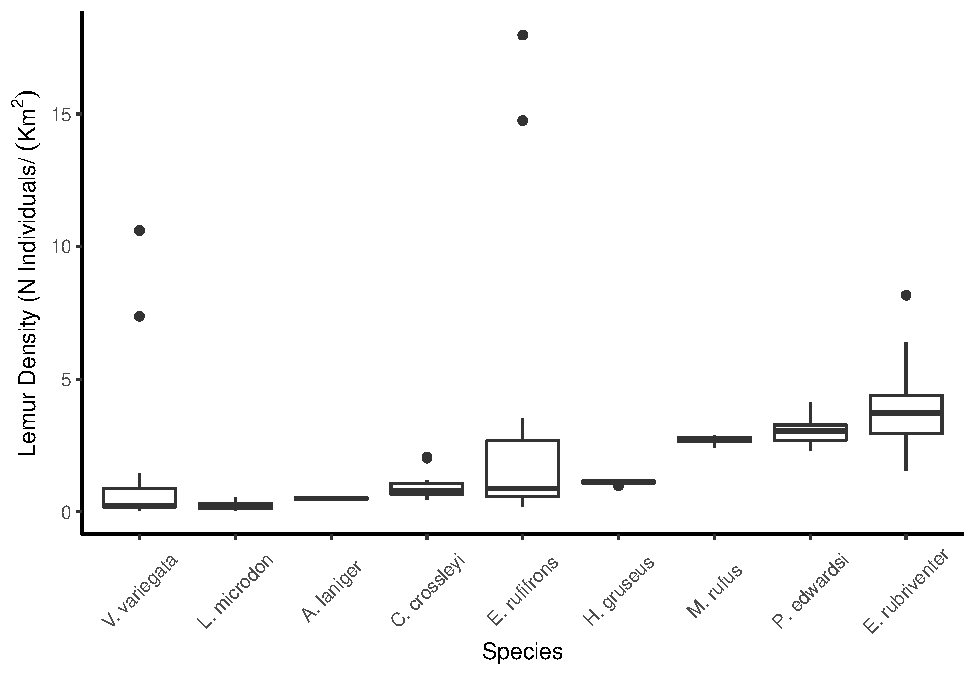
\includegraphics{project_draft_2_files/figure-latex/unnamed-chunk-10-1.pdf}
\caption{Boxplot of lemur densities for each species surveyed.}
\end{figure}

\hypertarget{question-2-what-variables-are-related-to-differences-in-lemur-densities-1}{%
\subsection{Question 2: What variables are related to differences in
lemur
densities?}\label{question-2-what-variables-are-related-to-differences-in-lemur-densities-1}}

Our best model with site as an independent vaiable demonstrates that
fruit nitrogen content, latitude, roughness, slope, fruit length, fruit
width, and the sites were significantly related to lemur density. This
model explains 46.7\% of the variance in lemur density. With every
increase in one percentage of nitrogen on the log scale, lemur density
increases by 11.310 individuals per square Km (p = 0.007). With every
increase in one degree latitude, lemur density decreases by 28.030
individuals per square Km (p = 0.021). With every increase in one
roughness unit, lemur density decreases by 0.007 individuals per square
Km (p = 0.0.021). With every increase in one degree in slope, lemur
density increases by 0.259 individuals per square Km (p = 0.0294). Site
Maharira has 8.080 fewer lemurs per square Km (p = 0.275) when compared
to Ampatsoana, whereas Valohoaka has 7.845 fewer (p = 0.0182) and
Vohiparara has 6.291 fewer (0.02026). With every increase in one mm of
mean fruit length on the log scale, lemur density increases by 8.711
individuals per square Km (p = 0.009). On the other hand, with every
increase in one mm of mean fruit width on the log scale, lemur density
decreases by 10.070 individuals per square Km (p = 0.002).

When we included site as a random variable, only nitrogen content, fruit
length, and fruit width were significantly related to lemur densities in
the best model. However, this model explained less variation in lemur
density (43.580\%) than the model where it was included as an
independent variable. With every increase in one percentage of mean
nitrogen on the log scale, lemur density increases by 7.758 individuals
per square Km (p = 0.002). With every increase in one mm of the mean
fruit length, lemur density increases by 7.737 individuals per square Km
(p = 0.00483). With every increase in one mm of the mean fruit width,
lemur density decreases by 6.512 individuals per square Km (p = 0.0117).
Data visualization of the relationships between key habitat variables
and lemur densities are found on the R Shinp application.

\hypertarget{question-3-what-transect-level-characteristics-and-plant-functional-traits-are-related-to-the-density-of-individual-lemur-species-1}{%
\subsection{Question 3: What transect-level characteristics and plant
functional traits are related to the density of individual lemur
species?}\label{question-3-what-transect-level-characteristics-and-plant-functional-traits-are-related-to-the-density-of-individual-lemur-species-1}}

In our species-specific models, we identified that lemur species differ
in their relationships to the habitat variables. Based on our best model
for \emph{Avahi laniger}, we found that log seed length, latitude, log
seed width, log SLA, site Maharira, site Valohoaka, site Vohiparara, log
fruit length, and log fruit width were related to the density of Avahi
laniger (p \textless{} 0.001). This model explains 82.4\% of variation
in density. The model for the \emph{Eulemur rubriventer} species
indicated that log nitrogen, log SLA, slope, SiteMaharira,
SiteMiaranony, SiteValohoaka (marginally), Site Vohiparara, log fruit
length, and log fruit width are relevant to \emph{Eulemur rubriventer}
densities (p = 0.002). This model explains 56.95\% of the variation in
the density data. The model for Lepilemur microdon indicated that log
nitrogen, log tannins (marginally), log SLA, slope, site Maharira, site
Valohoaka, log fruit length, and log fruit width are significantly
related to the density of this species (p \textless{} 0.001). The model
explained 97.13\% of the variability in density. The model for
\emph{Propithecus edwardsi} indicated that latitude, log seed width, log
tannins, longitude, site Maharira, site Miaranony, siteValohoaka,
siteVohiparara, log fruit length, and log fruit width are relevant to
the densities of the species (p \textless{} 0.001). This model explained
about 75\% of the variability in the density of the species (Adjusted
R-squared: 0.7452). Again, data visualization of the relationships
between key habitat variables and lemur densities are found on the R
Shinp application.

\hypertarget{summary-and-conclusions}{%
\section{Summary and Conclusions}\label{summary-and-conclusions}}

There is a significant difference in Lemur population density between
different species and between different sites. Although Miaranony and
Valohoaka have greater lemur densities than the other sites, this is
likely driven by outliers. Because Valohoaka is primary forest whereas
Ampastona and Vohiparara are disturbed, secondary forests, human
disturbances could be a driving force of this pattern. Ampatsoana,
Maharira, and Vohiparara all have similar lemur densities. \emph{Eulemur
rubriventer, Propithecus edwardsi}, and \emph{Microcebus rufus} all tend
to have higher densities than the other lemur species, whereas
\emph{Varecia variegata, Lepilemur microdon, Avahi laniger}, and
\emph{Cheirogaleus crossleyi} tend to have lower densities. Because
\emph{M. rufus} and \emph{C. crossleyi} are the two mouse lemur species
in the dataset, it is surprising that they are in different groups based
on their densities, and it could be because \emph{M. rufus} is
resilient, even potentially preferential, to human-disturbed areas
(Herrera et al.~2011).

Our analyses demonstrate that these differences in densities are related
to various transect level variables, such as fruit length, nitrogen
content, and fruit width. Latitude, roughness, slope, and site also may
be relevant, as indicated by the best linear model created using species
and transect site as the only random effects. These results highlight
the potential importance of plant functional traits in driving patterns
of lemur density across a landscape. This is consistent with the
literature; for example, lemur population sizes are known to be related
to the presence of fruiting trees (Herrera et al.~2018). Latitude,
roughness, and slope could influence which plant species occur in
different sites. However, differences in densities could also be
reflective of life history characteristics or other variables that were
not included in this study, such as human disturbance.

Our analyses highlighted variation in the variables related to lemur
density between the various lemur species. However, fruit width and
fruit length are related to the densities of each of the four species we
analyzed in depth. Fruit characteristics such as tannin concentration,
seed length, and seed width were relevant to the densities of certain
lemur species, but they were not significantly related to the densities
of other lemur species. Similarly, landscape characteristics such as
slope and latitude were found to be related to the densities of certain
lemur species. The differences between the models of the individual
lemur species suggests that traits of the lemurs might also be important
in determining what habitat variables relate to their densities. Lemurs
vary greatly in their diets, habitat preferences, and foraging ecology,
and lemur social structure is related to ecological variables (Overdorff
1996).

These results could have management implications. For example, it could
be beneficial to focus tree restoration efforts on species that contain
the traits that are positively related to lemur densities, such as
nitrogen content. In fact, restoration schemes based on lemur feeding
trees have already been proposed in Madagascar (Steffens et al.~2020).
Fruit length and fruit width are also related to lemur densities,
although further studies would be needed to determine which fruit sizes
and lengths best support various lemur species. Information on the
length and width of fruit from trees could be used to make strategic
decisions to best support the populations of specific lemur species.

Future studies ought to integrate other variables into the analysis of
the three questions posed in this project. For example, other studies
could investigate how functional traits and climatic variables interact
with anthropogenic disturbance to drive patterns in lemur densities.
Human disturbance is known to impact mammal population densities in the
neotropics (Tucker et al.~2021), so there might be similar dynamics in
Madagascar. It would also be interesting to incorporate lemur functional
traits to analyze if lemur diets, body sizes, and behavioral traits are
significantly related to their densities in a given area. Furthermore, a
similar study at a larger scale could be interesting because mouse lemur
densities are related to biogeographical variables (Setash et al.~2017),
so it would be interesting to identify the biogeogrphical variables that
are related to other species.

\newpage

\hypertarget{references}{%
\section{References}\label{references}}

Barton, K. (2020). MuMIn: Multi-Model Inference. R package version
1.43.17. \url{https://CRAN.R-project.org/package=MuMIn}

Bates, D., Maechler, M., Bolker, B., Walker, S. (2015). Fitting Linear
Mixed-Effects Models Using lme4. Journal of Statistical Software, 67(1),
1-48. \url{doi:10.18637/jss.v067.i01}

Brown, K. A., Parks, K. E., Bethell, C. A., Johnson, S. E., \& Mulligan,
M. (2015). Predicting Plant Diversity Patterns in Madagascar:
Understanding the Effects of Climate and Land Cover Change in a
Biodiversity Hotspot. PLOS ONE, 10(4), e0122721.
\url{https://doi.org/10.1371/journal.pone.0122721}

De Mendiburu, F. (2020). agricolae: Statistical Procedures for
Agricultural Research. R package version 1.3-3.
\url{https://CRAN.R-project.org/package=agricolae}

Donati, G., Santini, L., Eppley, T. M., Arrigo-Nelson, S. J., Balestri,
M., Boinski, S., Bollen, A., Bridgeman, L. L., Campera, M., Carrai, V.,
Chalise, M. K., Derby Lewis, A., Hohmann, G., Kinnaird, M. F., Koenig,
A., Kowalewski, M., Lahann, P., McLennan, M. R., Nekaris, A. K. I.,
\ldots{} Ganzhorn, J. U. (2017). Low Levels of Fruit Nitrogen as Drivers
for the Evolution of Madagascar's Primate Communities. Scientific
Reports, 7(1), 14406. \url{https://doi.org/10.1038/s41598-017-13906-y}

Fiske, I., Chandler, R. (2011). unmarked: An R Package for Fitting
Hierarchical Models of Wildlife Occurrence and Abundance. Journal of
Statistical Software, 43(10), 1-23. URL
\url{http://www.jstatsoft.org/v43/i10/}.

Herrera, J. P., Wright, P. C., Lauterbur, E., Ratovonjanahary, L., \&
Taylor, L. L. (2011). The Effects of Habitat Disturbance on Lemurs at
Ranomafana National Park, Madagascar. International Journal of
Primatology, 32(5), 1091--1108.
\url{https://doi.org/10.1007/s10764-011-9525-8}

Herrera, J. P., Borgerson, C., Tongasoa, L., Andriamahazoarivosoa, P.,
Rasolofoniaina, B. J. R., Rakotondrafarasata, E. R., Randrianasolo, J.
L. R. R., Johnson, S. E., Wright, P. C., \& Golden, C. D. (2018).
Estimating the population size of lemurs based on their mutualistic food
trees. Journal of Biogeography, 45(11), 2546--2563.
\url{https://doi.org/10.1111/jbi.13409}

Kuznetsova, A., Brockhoff, P.B., Christensen, R.H.B. (2017). ``lmerTest
Package: Tests in Linear Mixed Effects Models.'' \emph{Journal of
Statistical Software}, \emph{82}(13), 1-26. doi: 10.18637/jss.v082.i13
(URL: \url{https://doi.org/10.18637/jss.v082.i13}).

Lim, J. Y., Svenning, J.-C., Göldel, B., Faurby, S., \& Kissling, W. D.
(2020). Frugivore-fruit size relationships between palms and mammals
reveal past and future defaunation impacts. Nature Communications,
11(1), 4904. \url{https://doi.org/10.1038/s41467-020-18530-5}

Park, D. S., \& Razafindratsima, O. H. (2019). Anthropogenic threats can
have cascading homogenizing effects on the phylogenetic and functional
diversity of tropical ecosystems. Ecography, 42(1), 148--161.
\url{https://doi.org/10.1111/ecog.03825}

Overdorff, D. J. (1996). Ecological correlates to social structure in
two lemur species in Madagascar. American Journal of Physical
Anthropology, 100(4), 487--506.
\url{https://doi.org/10.1002/(SICI)1096-8644(199608)100:4}\textless487::AID-AJPA4\textgreater3.0.CO;2-O

Razafindratsima, O. H., Mehtani, S., \& Dunham, A. E. (2013).
Extinctions, traits and phylogenetic community structure: Insights from
primate assemblages in Madagascar. Ecography, 36(1), 47--56.
\url{https://doi.org/10.1111/j.1600-0587.2011.07409.x}

Schwitzer, C., Mittermeier, R. A., Johnson, S. E., Donati, G., Irwin,
M., Peacock, H., \ldots{} \& Wright, P. C. (2014). Averting lemur
extinctions amid Madagascar's political crisis. Science, 343(6173),
842-843.

Setash, C. M., Zohdy, S., Gerber, B. D., \& Karanewsky, C. J. (2017). A
biogeographical perspective on the variation in mouse lemur density
throughout Madagascar. Mammal Review, 47(3), 212--229.
\url{https://doi.org/10.1111/mam.12093}

Steffens, K. J. E. (2020). Lemur food plants as options for forest
restoration in Madagascar. Restoration Ecology, 28(6), 1517--1527.
\url{https://doi.org/10.1111/rec.13234}

Valenta, K., Burke, R. J., Styler, S. A., Jackson, D. A., Melin, A. D.,
\& Lehman, S. M. (2013). Colour and odour drive fruit selection and seed
dispersal by mouse lemurs. Scientific Reports (Nature Publisher Group),
3, 2424. \url{http://dx.doi.org.proxy.lib.duke.edu/10.1038/srep02424}

Wright, P., Razafindratsita, V., Pochron, S., \& Jernvall, J. (1970).
The Key to Madagascar Frugivores. In Tropical Fruits and Frugivores: The
Search for Strong Interactors (pp.~121--138).
\url{https://doi.org/10.1007/1-4020-3833-X_7}

Zeileis, A. Hothorn, T. (2002). Diagnostic Checking in Regression
Relationships. R News 2(3), 7-10. URL
\url{https://CRAN.R-project.org/doc/Rnews/}

Wickham, H. ggplot2: Elegant Graphics for Data Analysis. Springer-Verlag
New York, 2016.

\end{document}
